% !TEX root =  ../main_manuscript.tex 
\section{Personalized Schedule of Invasive Tests for Detecting Progression} 
\label{sec:schedule}

\subsection{Cumulative-risk of progression} 
\label{subsec:cum_risk}
Using the joint model fitted to the available data $\mathcal A_n$, we aim to derive a personalized schedule of invasive tests for a new patient $j$. The basis for our calculations is the dynamic cumulative risk function. In particular, we let $t$ denote the last time an invasive test was performed and $v$ the current visit time. As in our motivating example, we allow that longitudinal biomarker information can be collected after the last invasive test, i.e., $v \geq t$ (i.e., see Figure~\ref{fig:dynrisk_explanation}). The patient-specific cumulative-risk of progression at future time $u$ is defined as:
\begin{eqnarray}
\label{eq:cumulative_risk}
\nonumber \lefteqn{R_j(u \mid t, v) = \mbox{Pr}\big\{T^*_j \leq u \mid T^*_j > t, \mathcal{Y}_{1j}(v), \ldots, \mathcal{Y}_{Kj}(v), \mathcal{A}_n\big\}}\\
\nonumber & = & \int \int \mbox{Pr}(T^*_j \leq u \mid T^*_j > t, \boldsymbol{b}_{j}, \boldsymbol{\theta}) \; p\big\{\boldsymbol{b}_j \mid T^*_j > t, \mathcal{Y}_{1j}(v), \ldots, \mathcal{Y}_{Kj}(v), \boldsymbol{\theta} \big\}\\
& & \quad \quad \times \; p(\boldsymbol{\theta} \mid \mathcal{A}_n) \; \mathrm{d}\boldsymbol{b}_j \mathrm{d}\boldsymbol{\theta}, \quad u \geq t,
\end{eqnarray}
where $\{\mathcal{Y}_{1j}(v), \ldots, \mathcal{Y}_{Kj}(v)\}$ denotes the history of observed longitudinal outcomes until the current visit time $v$. The cumulative risk function $R_j(\cdot)$ dynamically updates over time as more longitudinal data becomes available (Panel~B~and~C, Figure~\ref{fig:dynrisk_explanation}).
\begin{figure}
\centerline{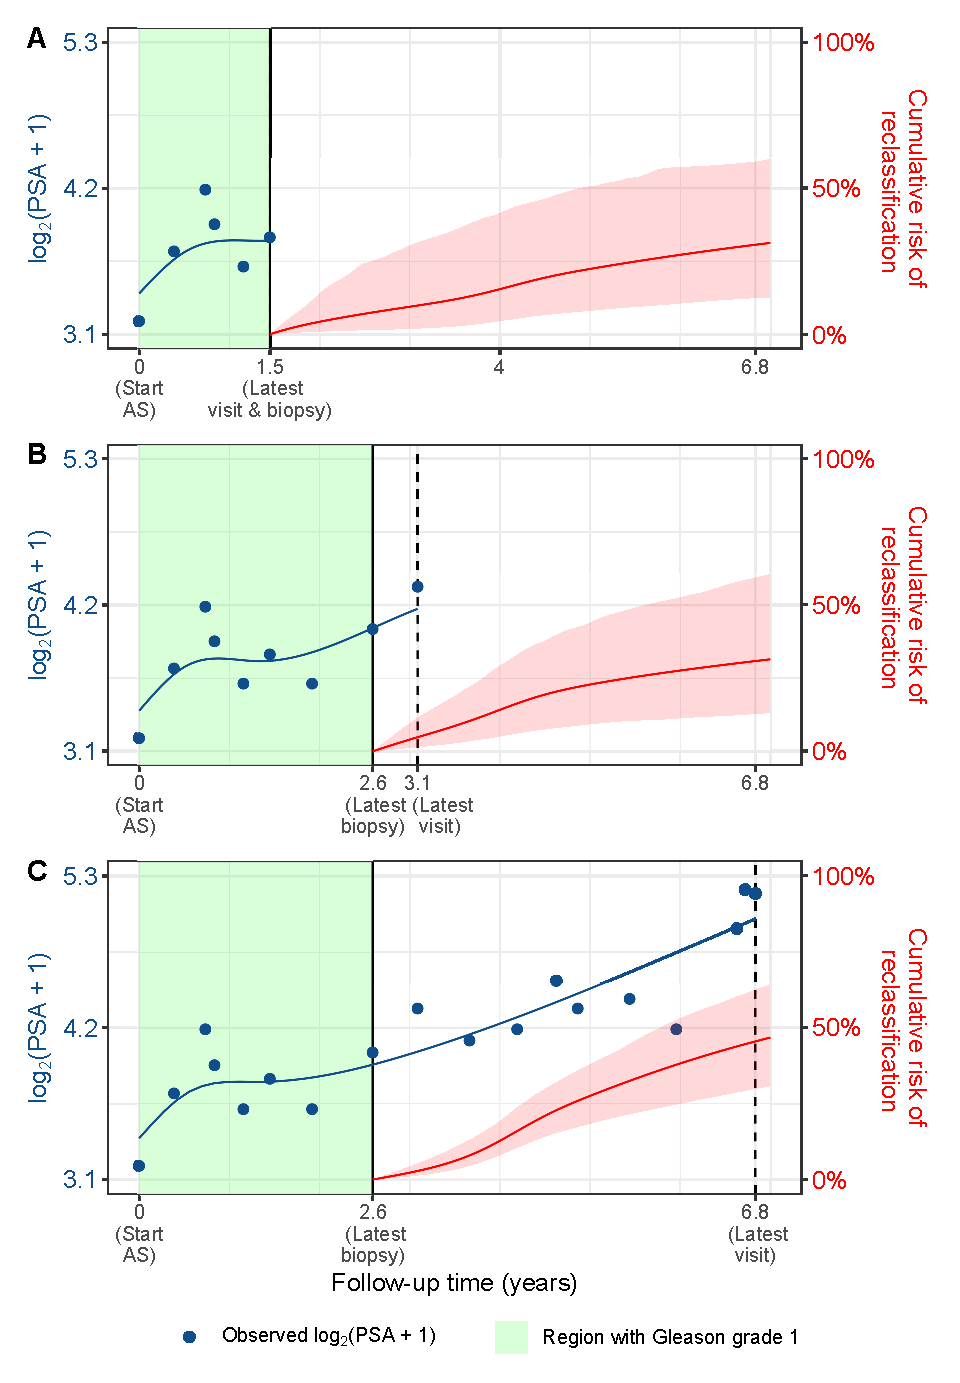
\includegraphics{images/dynrisk_plot_102.eps}}
\caption{\textbf{Cumulative-risk of progression changing dynamically over follow-up} as more patient data is gathered. A single longitudinal outcome, namely, a continuous biomarker of disease progression, is used for illustration. \textbf{Panels~A,~B~and~C:} are ordered by the time of the current visit (dashed vertical black line) of a new patient. At each of these visits, we combine the accumulated longitudinal measurements (shown in blue), and last time of negative invasive test (solid vertical green line) to obtain the updated cumulative-risk profile (shown in red) of the patient. All values are illustrative.} 
\label{fig:dynrisk_explanation}
\end{figure}

\subsection{Personalized Decision Rule} 
\label{subsec:pers_schedule}
Our aim is to employ the cumulative-risk function $R_j(\cdot)$ to develop a risk-based personalized schedule of invasive tests for the $j$-th patient. Typically, the decision to perform such an invasive procedure takes place at the same visit times at which auxiliary data (e.g., biomarkers) are measured. We let $U = \{u_1, \ldots, u_L\}$ represent the schedule of such visits (e.g., every six months in prostate cancer for PSA measurement), where $u_1 = v$ is the the current visit time. The last time $u_L$ is selected according to the information we have available in the original dataset $\mathcal A_n$. That is, we will only plan tests for the future patient $j$ up to the follow-up time $u_L$ at which we had sufficient number of events in $\mathcal A_n$ (e.g., up to the 80\% or 90\% percentile of progression times). 

We propose to take the decision of conducting a test at a future visit time $u_l \in U$ when the cumulative risk of progression exceeds a certain threshold $\kappa$, i.e.,
\[
Q_j^\kappa (u_l \mid t_l, v) = I \big \{ R_j(u_l \mid t_l, v) \geq \kappa \big\}, \quad 0 \leq \kappa \leq 1,
\]
where $I(\cdot)$ denotes the indicator function. The time point $t_l$ is the time point the last invasive test was performed, i.e., if a test gets planned at time $u_l$, then the successive test decision at time $u_{l+1}$ is made using an updated cumulative-risk profile (Figure~\ref{fig:schedule_explanation}). This updated cumulative-risk profile accounts for the possibility that progression may occur after time $u_l < T^*_j$. Hence, the definition of $t_l$ is
\[
t_l = \left \{ 
\begin{array}{ll}
t, & \mbox{if } l = 1\\
t_{l-1}, & \mbox{if } l \geq 2 \mbox{ and } Q_j^\kappa (u_{l-1} \mid t_{l-1}, v) = 0\\
u_{l-1}, & \mbox{if } l \geq 2 \mbox{ and } Q_j^\kappa (u_{l-1} \mid t_{l-1}, v) = 1\\
\end{array}
\right.
\]
We should note that for all the future decisions we use only the longitudinal information that we have collected up to the current visit $v = u_1$.

\subsection{Expected Number of Tests and Time Delay in Detecting Progression}
\label{subsec:exp_delay_estimation}
To facilitate shared-decision making, we translate our proposed decision rule, i.e., the choice of a specific $\kappa$, into clinically relevant quantities. Namely, for the specific $\kappa$ value we have selected, we would like to know how many tests we expect to perform in the future for patient $j$, and if he/she progresses, what will be the expected delay in finding this progression. As explained before, the more tests, the shorter the delay will be but at the expense of increasing patient burden.

To calculate the expected number of tests and expected delay, we first suppose that patient $j$ never progressed in the period $[t, u_L]$. Under this assumption, the subset of future time points in $U$ at which a test is to be performed results into a personalized schedule of planned future tests, given by:
\begin{equation}
\label{eq:personalized_schedule_grid}
\{s_1, \ldots, s_{N_j}\} = \big\{ u_l \in U : Q_j^\kappa(u_l \mid t_l, v) = 1 \big\}, \quad N_j \leq L.
\end{equation}
Figure~\ref{fig:schedule_explanation} depicts this schedule for a hypothetical patient and risk threshold of 12\%.
\begin{figure}
\centerline{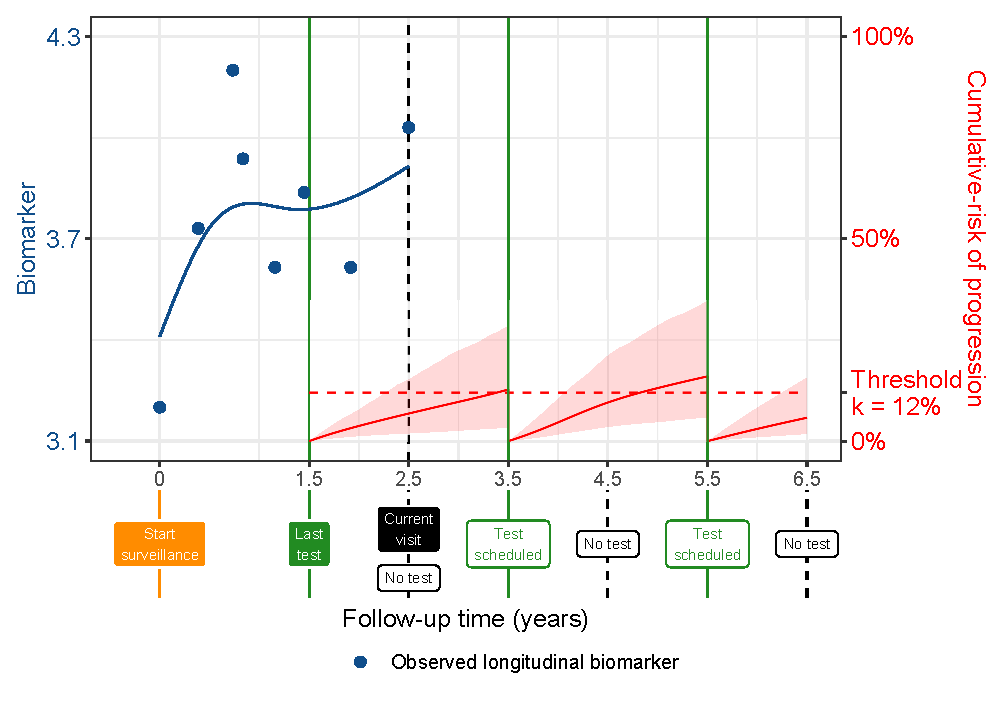
\includegraphics{images/schedule_explanation_102.eps}}
\caption{\textbf{Personalized Invasive Test Schedule Using Patient-specific Conditional Cumulative-risk of Progression}.  A single longitudinal outcome, namely, a continuous biomarker (observed: blue dots, fitted: blue line) of disease progression is used for illustration. The last test on which progression was not observed was conducted at $t=1.5$ years. The current visit time of the patient is $v=2.5$ years. Decisions for invasive test need to be made at a gap of every one year starting from the current visit until a horizon of 6.5 years. That is, $U=\{2.5, 3.5, 4.5, 5.5, 6.5\}$ years. Based on an example risk threshold of 12\% ($\kappa=0.12$) the future test decisions at time points in $U$ lead to a personalized schedule $S_j^{\kappa^*} (U \mid t=1.5, v=2.5) = \{3.5, 5.5\}$ years. The conditional cumulative-risk profiles $R_j(u_l \mid t_l, v)$ employed in~(\ref{eq:personalized_decision_grid}) are shown with red line (confidence interval shaded). It is called `conditional' because, for example, the second test at future time 5.5 years, is scheduled after accounting for the possibility that progression (true time $T^*_j$) may not have occurred until the time of the previously scheduled test at time $T^*_j>3.5$ years. All values are illustrative.} 
\label{fig:schedule_explanation}
\end{figure}
If patient $j$ never progressed in the period $[t, u_L]$, as we initially supposed, we would conduct $N_j$ tests. However, if the patient did progress at some point $T_j^* < u_L$, then we will conduct less tests. We formally define the discrete random variable denoting the number of performed tests in conjunction with the true progression time $T_j^*$ as:
\[
\mathcal N_j (S^\kappa) = \left \{
\begin{array}{ll}
1, & \mbox{ if } \; t < T^*_j \leq s_1,\\
2, & \mbox{ if } \; s_1 < T^*_j \leq s_2,\\
\vdots&\\
N_j, & \mbox{ if } \; s_{N_j-1} < T^*_j \leq s_{N_j},
\end{array}
\right.
\]
where $S^\kappa = \{s_1, \ldots, s_{N_j}\}$. Then the expected number of future tests for patient $j$ will be the expected value of $\mathcal N_j (S^\kappa)$ that be calculated with the expression:
\begin{equation}
E \big \{\mathcal N_j(S^\kappa)\big\} = \sum_{n = 1}^{N_j} n \times \mbox{Pr}(s_{n-1} < T^*_j \leq s_n \mid T^*_j \leq s_{N_j}), \quad s_0 = t,
\label{eq:exp_tests}
\end{equation}
where 
\[
\mbox{Pr}(s_{n-1} < T^*_j \leq s_n \mid T^*_j \leq s_{N_j}) = \frac{R_j(s_n \mid t, v) - R_j(s_{n-1} \mid t, v)}{R_j(s_{N_j} \mid t, v)}.
\]

In an analogous manner we can define the expected delay in finding progression, under the assumption that progression has occurred before $u_L$. In particular, we first define the random variable that quantifies the time difference between the true progression time $T_j^*$ and the time of the test at which this progression will be observed, i.e.,
\[
\mathcal D_j (S^\kappa) = \left \{
\begin{array}{ll}
s_1 - T_j^*, & \mbox{ if } \; t < T^*_j \leq s_1,\\
s_2 - T_j^*, & \mbox{ if } \; s_1 < T^*_j \leq s_2,\\
\vdots&\\
s_{N_j} - T_j^*, & \mbox{ if } \; s_{N_j-1} < T^*_j \leq s_{N_j},
\end{array}
\right.
\]
The expected delay will be the expected value of $\mathcal D_j (S^\kappa)$ given by the expression:
\begin{equation}
E \big \{ \mathcal D_j(S^\kappa)\big\} = \sum_{n = 1}^{N_j} \Big\{s_n - E(T^*_j \mid s_{n-1}, s_n, v)\Big\} \times \mbox{Pr}(s_{n-1} < T^*_j \leq s_n\mid T^*_j \leq s_N),
\label{eq:exp_delay}
\end{equation}
where
\begin{eqnarray*}
\lefteqn{E(T^*_j \mid s_{n-1}, s_n, v) = s_{n-1}}\\
&& + \; \int_{s_{n-1}}^{s_n} \mbox{Pr}\Big\{T^*_j \geq u \mid s_{n-1} < T^*_j \leq s_n, \mathcal{Y}_{1j}(v), \ldots, \mathcal{Y}_{Kj}(v), \mathcal{A}_n\Big\} \; \mathrm{d}u,
\end{eqnarray*}
where $E(T^*_j \mid s_{n-1}, s_n, v)$ denotes the conditional expected time of progression for the scenario $s_{n-1} < T^*_j \leq s_n$, and is calculated as the area under the corresponding survival curve.

The personalized schedule in~(\ref{eq:personalized_schedule_grid}) is updated as more patient data becomes available over subsequent follow-up visits. The personalized expected number of tests and expected time delay in detecting progression have the advantage that they are updated over follow-up as more patient data becomes available. Since they can be calculated for any schedule, patients and doctors can utilize them to compare schedules before making a decision. Although, in order to have a fair comparison of time delays between different schedules for the same patient, a compulsory test at a common horizon time point should be planned in all schedules.

\subsection{How to Select the Risk Threshold $\kappa$}
The risk threshold $\kappa$ controls the timing and the total number of invasive tests in the personalized schedule $S^\kappa$. And through the timing and total number of planned tests, $\kappa$ also indirectly affects the time delay (Figure~\ref{fig:delay_explanation}) that may occur in detecting progression if a particular schedule is followed. Hence, $\kappa$ should be chosen while balancing both the number of invasive tests (burden) and the time delay in detecting progression (less is beneficial).

To facilitate the choice of $\kappa$ in practice, and in accordance to our developments in the previous section, we translate different choices for this parameter into the expected number of test and expected delay. More specifically, for a specific patient $j$ and at the current visit time $v$, we can construct the bi-dimensional Euclidean space of the expected total number of invasive tests (x-axis) and the corresponding expected time delay in detecting progression (y-axis) for test schedules planned by varying $\kappa$ in $[0, 1]$. An example of such a space is given in Figure~\ref{fig:kappa_choice}.
\begin{figure}
\centerline{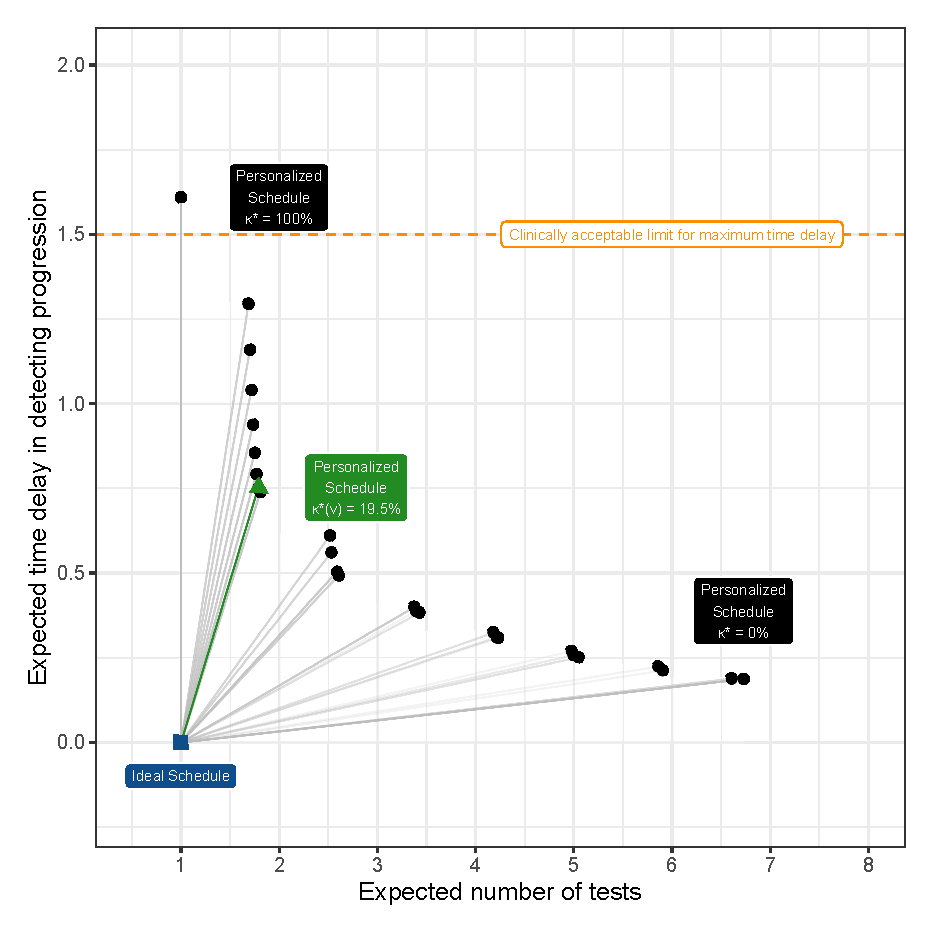
\includegraphics{images/kappa_choice_102.eps}}
\caption{\textbf{Automatic choice of risk threshold $0 \leq \kappa \leq 1$ using~(\ref{eq:kappa_choice})}. The ideal schedule of tests at point (1,0) is shown as a blue square. It plans exactly one invasive test at the true time of progression $T^*_j$ of a patient and hence leads to a zero time delay in detecting progression. Personalized schedules based on a grid of thresholds chosen between $0 \leq \kappa \leq 1$ are shown with black circles. Higher thresholds lead to fewer tests, but also higher expected time delay. We propose to choose the personalized schedule based on $\kappa^*(v)=9.5\%$ threshold (green triangle). This is because it has the least Euclidean distance (shown with a green line) to the ideal schedule. It is also possible to find the least distance under a certain clinically acceptable limit on time delay (orange dashed line), or number of tests.}
\label{fig:kappa_choice}
\end{figure}
The ideal schedule for this patient would be the one that has only one test conducted at exactly the true time of progression $T^*_j$. In other words, it will have zero time delay. If we would weigh delay and the number of tests as equally important, then we could select as the risk threshold $\kappa^*(v)$ at the current visit time $v$ the threshold that minimizes Euclidean distance between the ideal schedule, i.e., point (1, 0) and and the set of points representing the different personalized schedules $S^{\kappa}$ corresponding to various, i.e.,
\begin{equation}
\label{eq:kappa_choice}
\kappa^*(v) = \argmin_{0 \leq \kappa \leq 1} \sqrt{\Big[E\big\{\mathcal N_j(S^\kappa)\big\} - 1\Big]^2 + \Big[E\big\{\mathcal D_j(S^\kappa )\big\} - 0\Big]^2}.
\end{equation}
Additional consequences of following a particular schedule, such as (quality-adjusted) life-years saved, can also be accommodated in~(\ref{eq:kappa_choice}). This can be achieved by first setting a point of optimality in a higher dimensional Euclidean space of the aforementioned consequences, and then minimizing the Euclidean distance relative to this point of optimality.

An alternative approach is to constraint one of the two dimensions. For example, depending on the age of patient $j$, he together with his physician may be willing to schedule a maximum number of future tests or may be apprehensive about having an expected time delay higher than a certain number of months. In such situations, the Euclidean distance in~(\ref{eq:kappa_choice}) can be minimized under constraints on the expected number of tests and/or expected time delay (Figure~\ref{fig:kappa_choice}). An additional benefit of this approach is that it alleviates the issue that the time delay and the number of tests have different units of measurement~\cite{cook1994equivalence}.

